% !TeX root = ../Doc_especific_mse_anchovy.tex

La LGPA introdujo los PMP obligatorios, estos deben especificar los objetivos, las metas y el período para reconstruir o mantener las poblaciones de peces al nivel del RMS junto con las estrategias para alcanzar los objetivos y metas establecidos. El PMP para la anchoveta norte fue aprobado el 9 de abril del 2018 (Res.Ex. N$^\circ$ 1197). Este declara una serie de objetivos operacionales asociados a estándares de manejo (indicador y punto de referencia) con los cuales se debe medir el progreso de la pesquería como consecuencia de la aplicación de medidas y/o acciones de manejo. El PMP declara llevar y mantener el stock de anchoveta a un nivel que permita asegurar la sustentabilidad biológica del recurso. Para tal efecto, el objetivo N$^\circ$1.1 es llevar y mantener el recurso al RMS, y la medida de manejo asociada a este objetivo es establecer una CBA basada en los PBR's  de la Resolución Exenta N$^\circ$291 del año 2015.
\newline

Para el caso del stock de anchoveta del norte de Chile se establecieron proxies al RMS \citep{Paya2014}, los cuales fueron ratificados por el CCT-PP. Para la BDRMS se estableció un valor igual al 50\% de la BD0, y para la FRMS se estableció aquella mortalidad por pesca que en el largo plazo produce el 55\% de la biomasa desovante por recluta (F55\%BDPR). La regla de control para este objetivo es aplicar una mortalidad por pesca constante al nivel del RMS.
\newline

Dado que el stock compartido de anchoveta es manejado en forma independiente por cada país y no existe actualmente un manejo pesquero conjunto, es necesario asumir algunas suposiciones sobre el procedimiento de manejo para la pesquería peruana. Las recomendaciones de captura para la zona sur del Perú son frecuentemente realizadas por científicos del \textit{Instituto del Mar del Perú} (IMARPE), y en su última recomendación aplicaron el modelo de producción excedentaria de \cite{jj1969generalized} re-parametrizado, estocástico y diferenciable usando información anual de la biomasa acústica estimada para la zona sur y de las capturas \citep{produce2021}. Las recomendaciones de captura hechas por el IMARPE para la zona sur del Perú son equivalentes a una tasa de explotación cercana al 0.30. Entonces, para la pesquería peruana se asume una tasa de explotación constante igual a 0.3 y la CBA que los PM producirán será asignada a la pesquería chilena, y la captura adicional peruana corresponderá al supuesto descrito anteriormente. Los procedimientos de manejo identificados, a partir de las discusiones internas del taller y entre los miembros de la SUBPESCA, sobre las prioridades de los PM para la pesquería de anchoveta norte se identificaron los siguientes:  

\begin{itemize}
    \item \textbf{Sin captura}: Se evalúa el nivel de abundancia máximo y variabilidad en el reclutamiento que puede alcanzar el stock bajo una condición sin captura (ver Figura \ref{fig:figure6}). 
    \item \textbf{Conocimiento perfecto de la abundancia del stock}: Se considera una mortalidad por pesca al 55\% de la biomasa desovante por recluta (ver Figura \ref{fig:figure6}). 
\end{itemize}


\subsection{PM actual: No se ajusta del patrón retrospectivo para la CBA.}

La evaluación de stock de anchoveta es actualizada dos veces al año. La primera actualización ocurre en octubre de cada año (i) donde el stock es proyectado cuatro semestres haciendo un supuesto acerca de los reclutamientos diferenciados por semestre y la captura igual a la CBA del año i (la captura del primer semestre ha ocurrido y la del segundo semestre es la diferencia con respecto a la CBA del año i). La segunda actualización ocurre en marzo del año siguiente (i+1) con información completa del año anterior (i), donde el stock se proyecta dos semestres nuevamente haciendo un supuesto en los reclutamientos futuros diferenciados por semestre. Las recomendaciones de la CBA son realizadas en escala anual.

\subsection{PM actual con rho de Mohn – se ajusta el patrón retrospectivo para la CBA}

El procedimiento de manejo actual tiene un alto grado de incertidumbre, ya que en la segunda actualización la CBA depende de si el último reclutamiento estimado por el modelo de evaluación es penalizado o no. Esto se debe a que el modelo de evaluación actual presenta un patrón retrospectivo positivo en los reclutamientos \citep{espinola2023}. Anticipando a que este patrón sea incorporado en la proyección, se aplica el estadístico de rho de Mohn \citep{mohn1999retrospective,hurtado2015looking,huynh2022closed} para la estimación de la CBA. Durante la proyección del stock de anchoveta, los reclutamientos
estimados al último semestre se corrigen en base al parámetro de rho de Mohn: \todo{Supongo que aquí va algo que está pendiente}
\newline

Donde es el reclutamiento ajustado, es el último reclutamiento estimado por el modelo de evaluación,
y el estadístico rho de Mohn (\todo{Aquí va la cita?}) para el reclutamiento es calculado a partir de un análisis retrospectivo, el
cual consiste en ir eliminando series de datos hasta los últimos 5 años más recientes (en pasos anuales).
Las estimaciones de un modelo consistente a lo largo del tiempo (sin patrón retrospectivo) debería
tener un . El ajuste rho se realiza en ambos pasos de tiempo del procedimiento de manejo.
\newline

El modelo de evaluación utilizado en estos dos MP es el Modelo de Acondicionamiento Rápido (RCM),
codificado en TMB y distribuido en el paquete SAMtool de R, y es una aproximación de la evaluación
actual de anchoveta codificada en ADMB. No es técnicamente factible probar la evaluación actual en
una simulación de circuito cerrado debido al tiempo de ejecución del modelo. Dado el mismo conjunto
de datos, las tendencias y la magnitud de las estimaciones históricas de la biomasa desovante son
similares entre los dos modelos (Figura \ref{fig:RCM_.ADMB}). Es importante destacar que RCM tiene el mismo
comportamiento retrospectivo (Figura \ref{fig:Retros_RCM}) que el modelo base de evaluación de stock.

\begin{figure}[H]
    \centering
    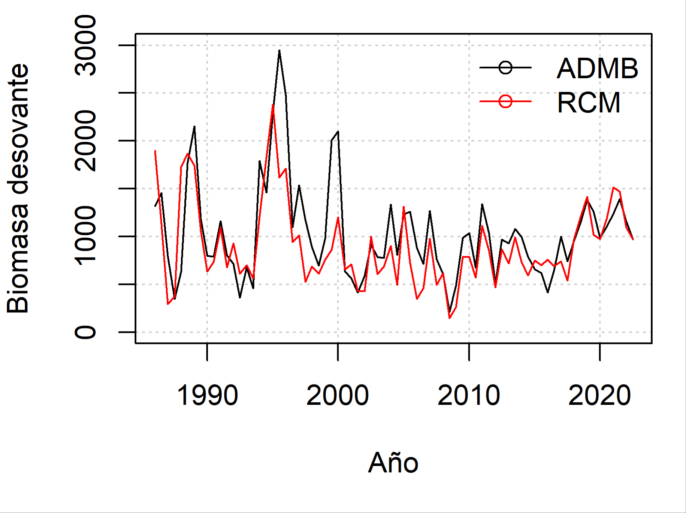
\includegraphics[scale=1.1]{RCM_.ADMB.pdf}  
    \caption{Comparación de la estimación de la biomasa desovante para el stock de anchoveta a través del
    Modelo de Acondicionamiento Rápido (RCM) y el modelo actual de evaluación en ADMB.}
    \label{fig:RCM_.ADMB}
\end{figure}  

\begin{figure}[H]
    \centering
    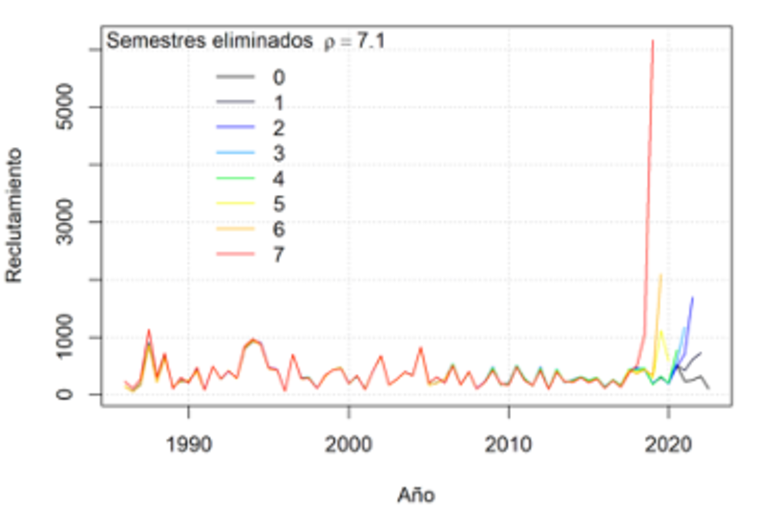
\includegraphics[scale=1.1]{Retros_RCM.pdf}  
    \caption{Patrón retrospectivo para el reclutamiento estimado para el Modelo de Acondicionamiento
    Rápido (RCM), se muestra el descuento de siete pasos de tiempo.}
    \label{fig:Retros_RCM}
\end{figure}  

\subsection{PM basado en una aproximación empírica, modelo basado simple.}

Este PM emplea la regla empírica propuesta por \cite{canales2021empirical} la que se basa en los valores de referencia en la captura y los valores de los cuantiles para la biomasa desovante estimada en el crucero de huevos. Los niveles de capturas representan los niveles históricos en las capturas semestrales de diferentes períodos.
\newline

Durante el taller presencial se acordó implementar esta regla de control usando tanto datos del crucero de huevos como del crucero acústico. El nivel de captura de referencia fue acordado para ambos casos como un valor de referencia de 285 mil toneladas, como representativo de los últimos años. Y los valores de los índices para cada caso corresponderá a los mismos criterios empleados por \cite{canales2021empirical}. 
\newline

\begin{figure}[H]
    \centering
    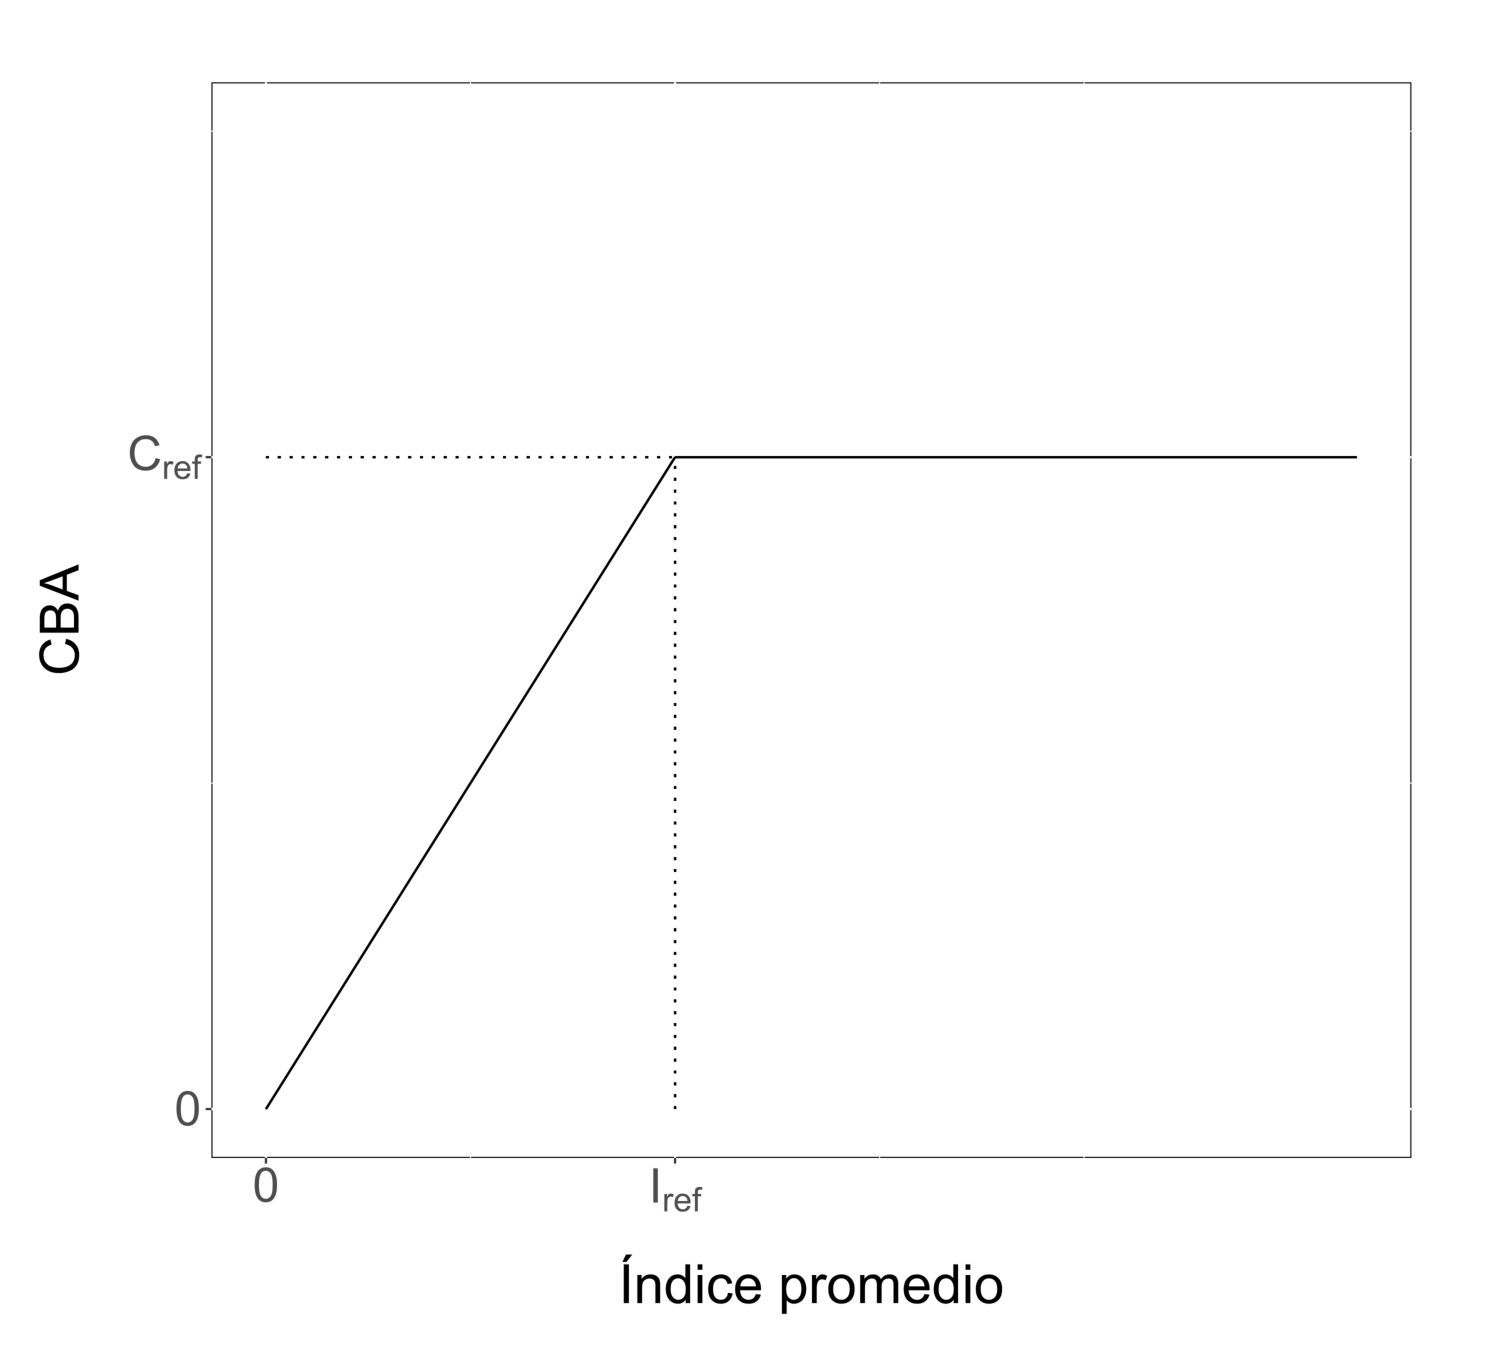
\includegraphics[scale=0.5]{cba_empirico.pdf}  
    \caption{Relación entre la captura de referencia y el índice de referencia para la regla de control de
    captura (RCC) basado en el crucero.}
    \label{fig:cba_empirico.pdf}
\end{figure} 
\todo{Ojo, esta imagen nunca se menciona en el texto}
% Con respecto a los reclutamientos se acordó: continuar con la metodología de utilizar el promedio diferenciado por semestre.

% \begin{itemize}
%     \item Para los PM establecidos se continuará con la metodología propuesta y usada habitualmente por el CCT-PP para proyectar el stock de anchoveta, promedios diferenciados por semestre \citep{espinola2023}. 
%     \item Para una futura exploración de PM se podrá explorar la inquietud señalada por la SUBPESCA, con relación a realizar un ejercicio con un sólo reclutamiento (como caso excepcional, por ejemplo, para escenarios del ENSO).
% \end{itemize}

En el Cuadro \ref{tab:tabla3} se resumen los diferentes procedimientos de manejo detallados anteriormente.

\begin{table}[H]
    \centering
    \caption{Resumen de los procedimientos de manejo en la simulación para la anchoveta norte. Las descripciones se entienden como variaciones del modelo operativo base por MO1.}
    \label{tab:tabla3}
    \begin{tabular}{|p{3.5cm}|p{10cm}|}
        \hline
        \textbf{Nombre} & \textbf{Descripción} \\
        \hline
        PM\_Actual & No se ajusta el patrón retrospectivo en el reclutamiento del último semestre.\\
        \hline
        PM\_Actual\_Rho & Se ajusta el patrón retrospectivo en el reclutamiento del último semestre.\\
        \hline
        PM\_empírico\_H & Se basa en el crucero de huevos. \\
        \hline
        PM\_empírico\_R & Se basa en el crucero acústico de reclutas. \\
        \hline
        Sin\_Captura & Procedimiento de referencia con F=0 \\
        \hline
        Manejo\_Perfecto & Procedimiento de referencia con conocimiento perfecto de la abundancia y puntos de referencia al RMS, F=55\%BDPR.\\
        \hline
    \end{tabular}
\end{table}


